\singlespace
\begin{savequote}[75mm] 
Resistance is not, then, in some limited sense a glorious banner of the past, but rather an unremitting struggle and a new consciousness in continuous development through subjective action, its aim being the objective process that leads to those ideals for which so many fell and continue even now to be murdered. \\
The musician too takes part in this fight. \\
\citeyearpar[Music and Revolution pp.273--274]{Nono}
\qauthor{Luigi Nono} 
\end{savequote}

\chapter{Appendix of Scores}
\doublespace
\newthought{The scores in this appendix} were each composed in 2018. Work on the compositions was begun and completed in a fairly rapid succession. As can be seen in the source code of appendix A, these pieces feature many organizational similarities. The compositions should not be considered as a cycle or series, but individual works that happen to share certain consistent principles.
\singlespace


\section{Scores}
\subsection{Cthar (for two cellos) Score}
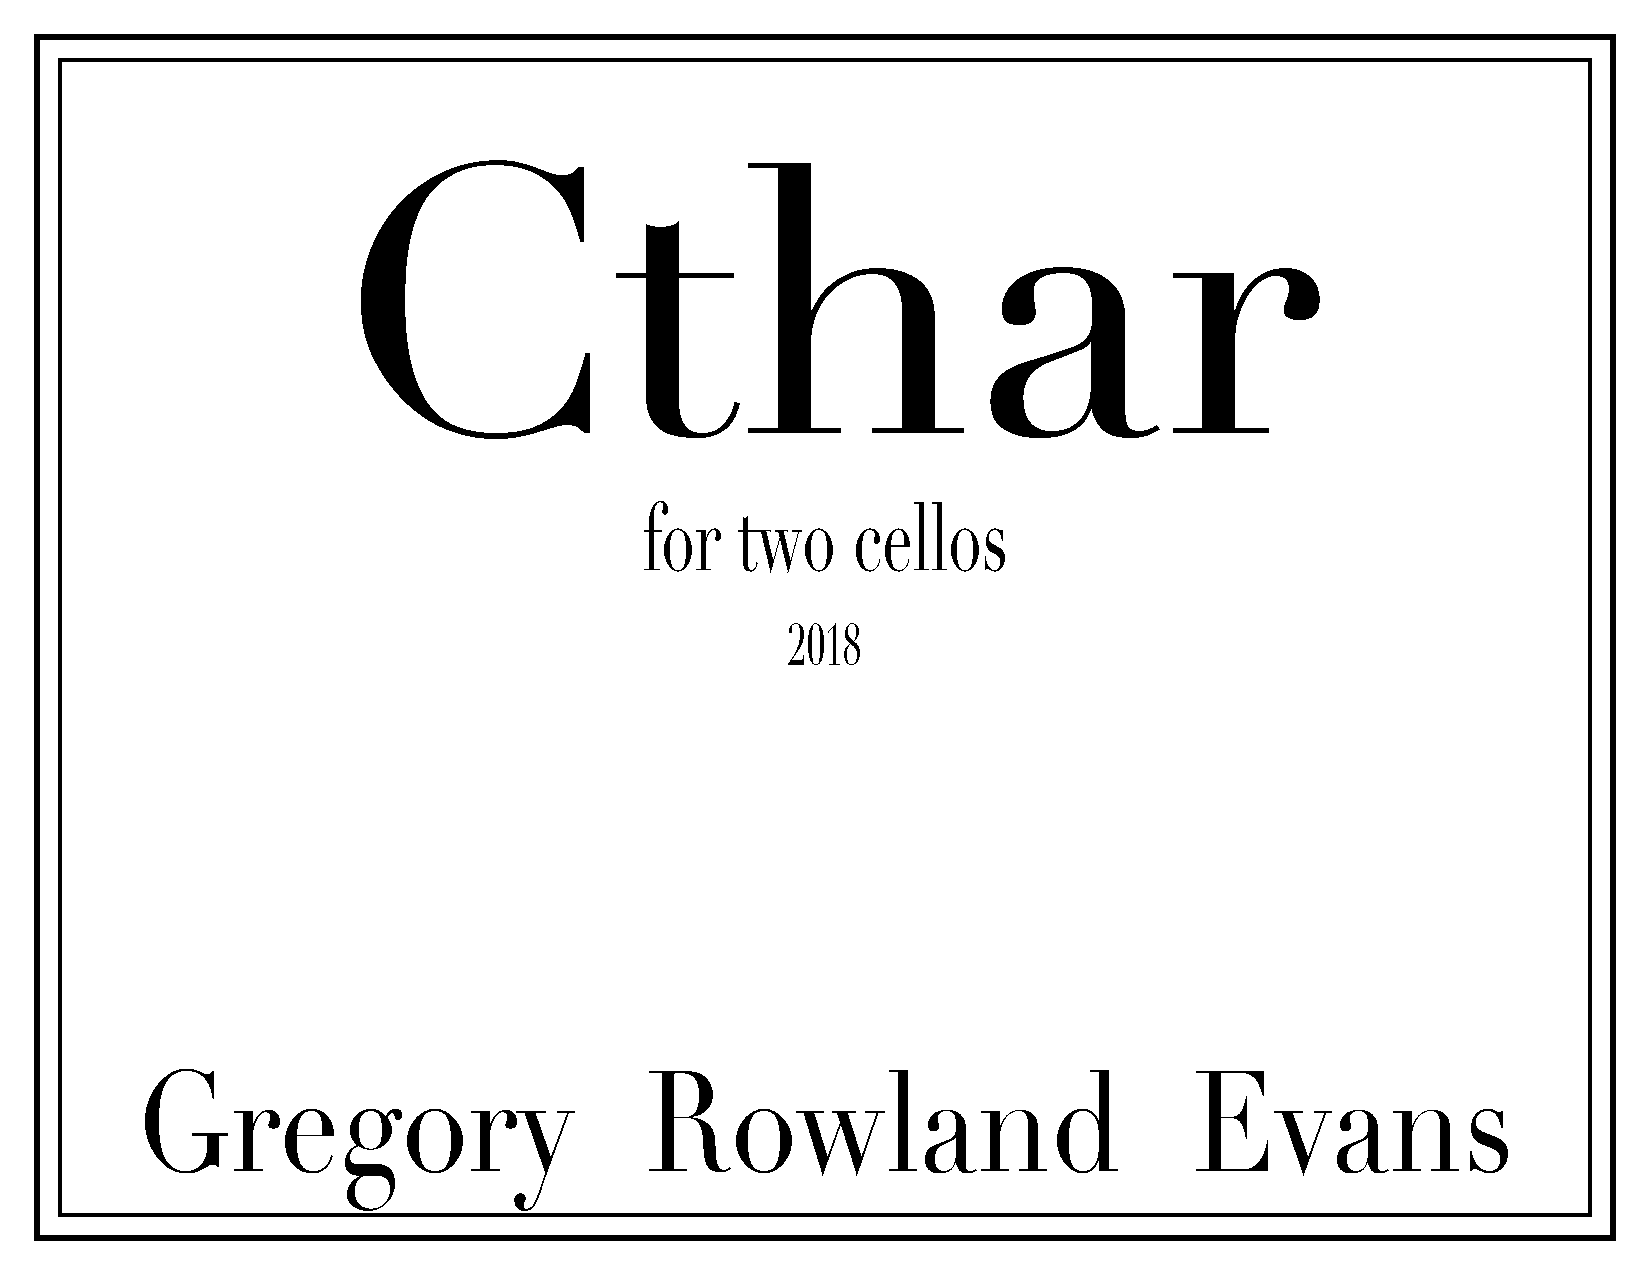
\includepdf[pages=-, pagecommand={}, width=7in,
  height=9.5in, keepaspectratio]{figures/Score/cthar_Score.pdf}

\subsection{Tianshu (for 12 players) Score}
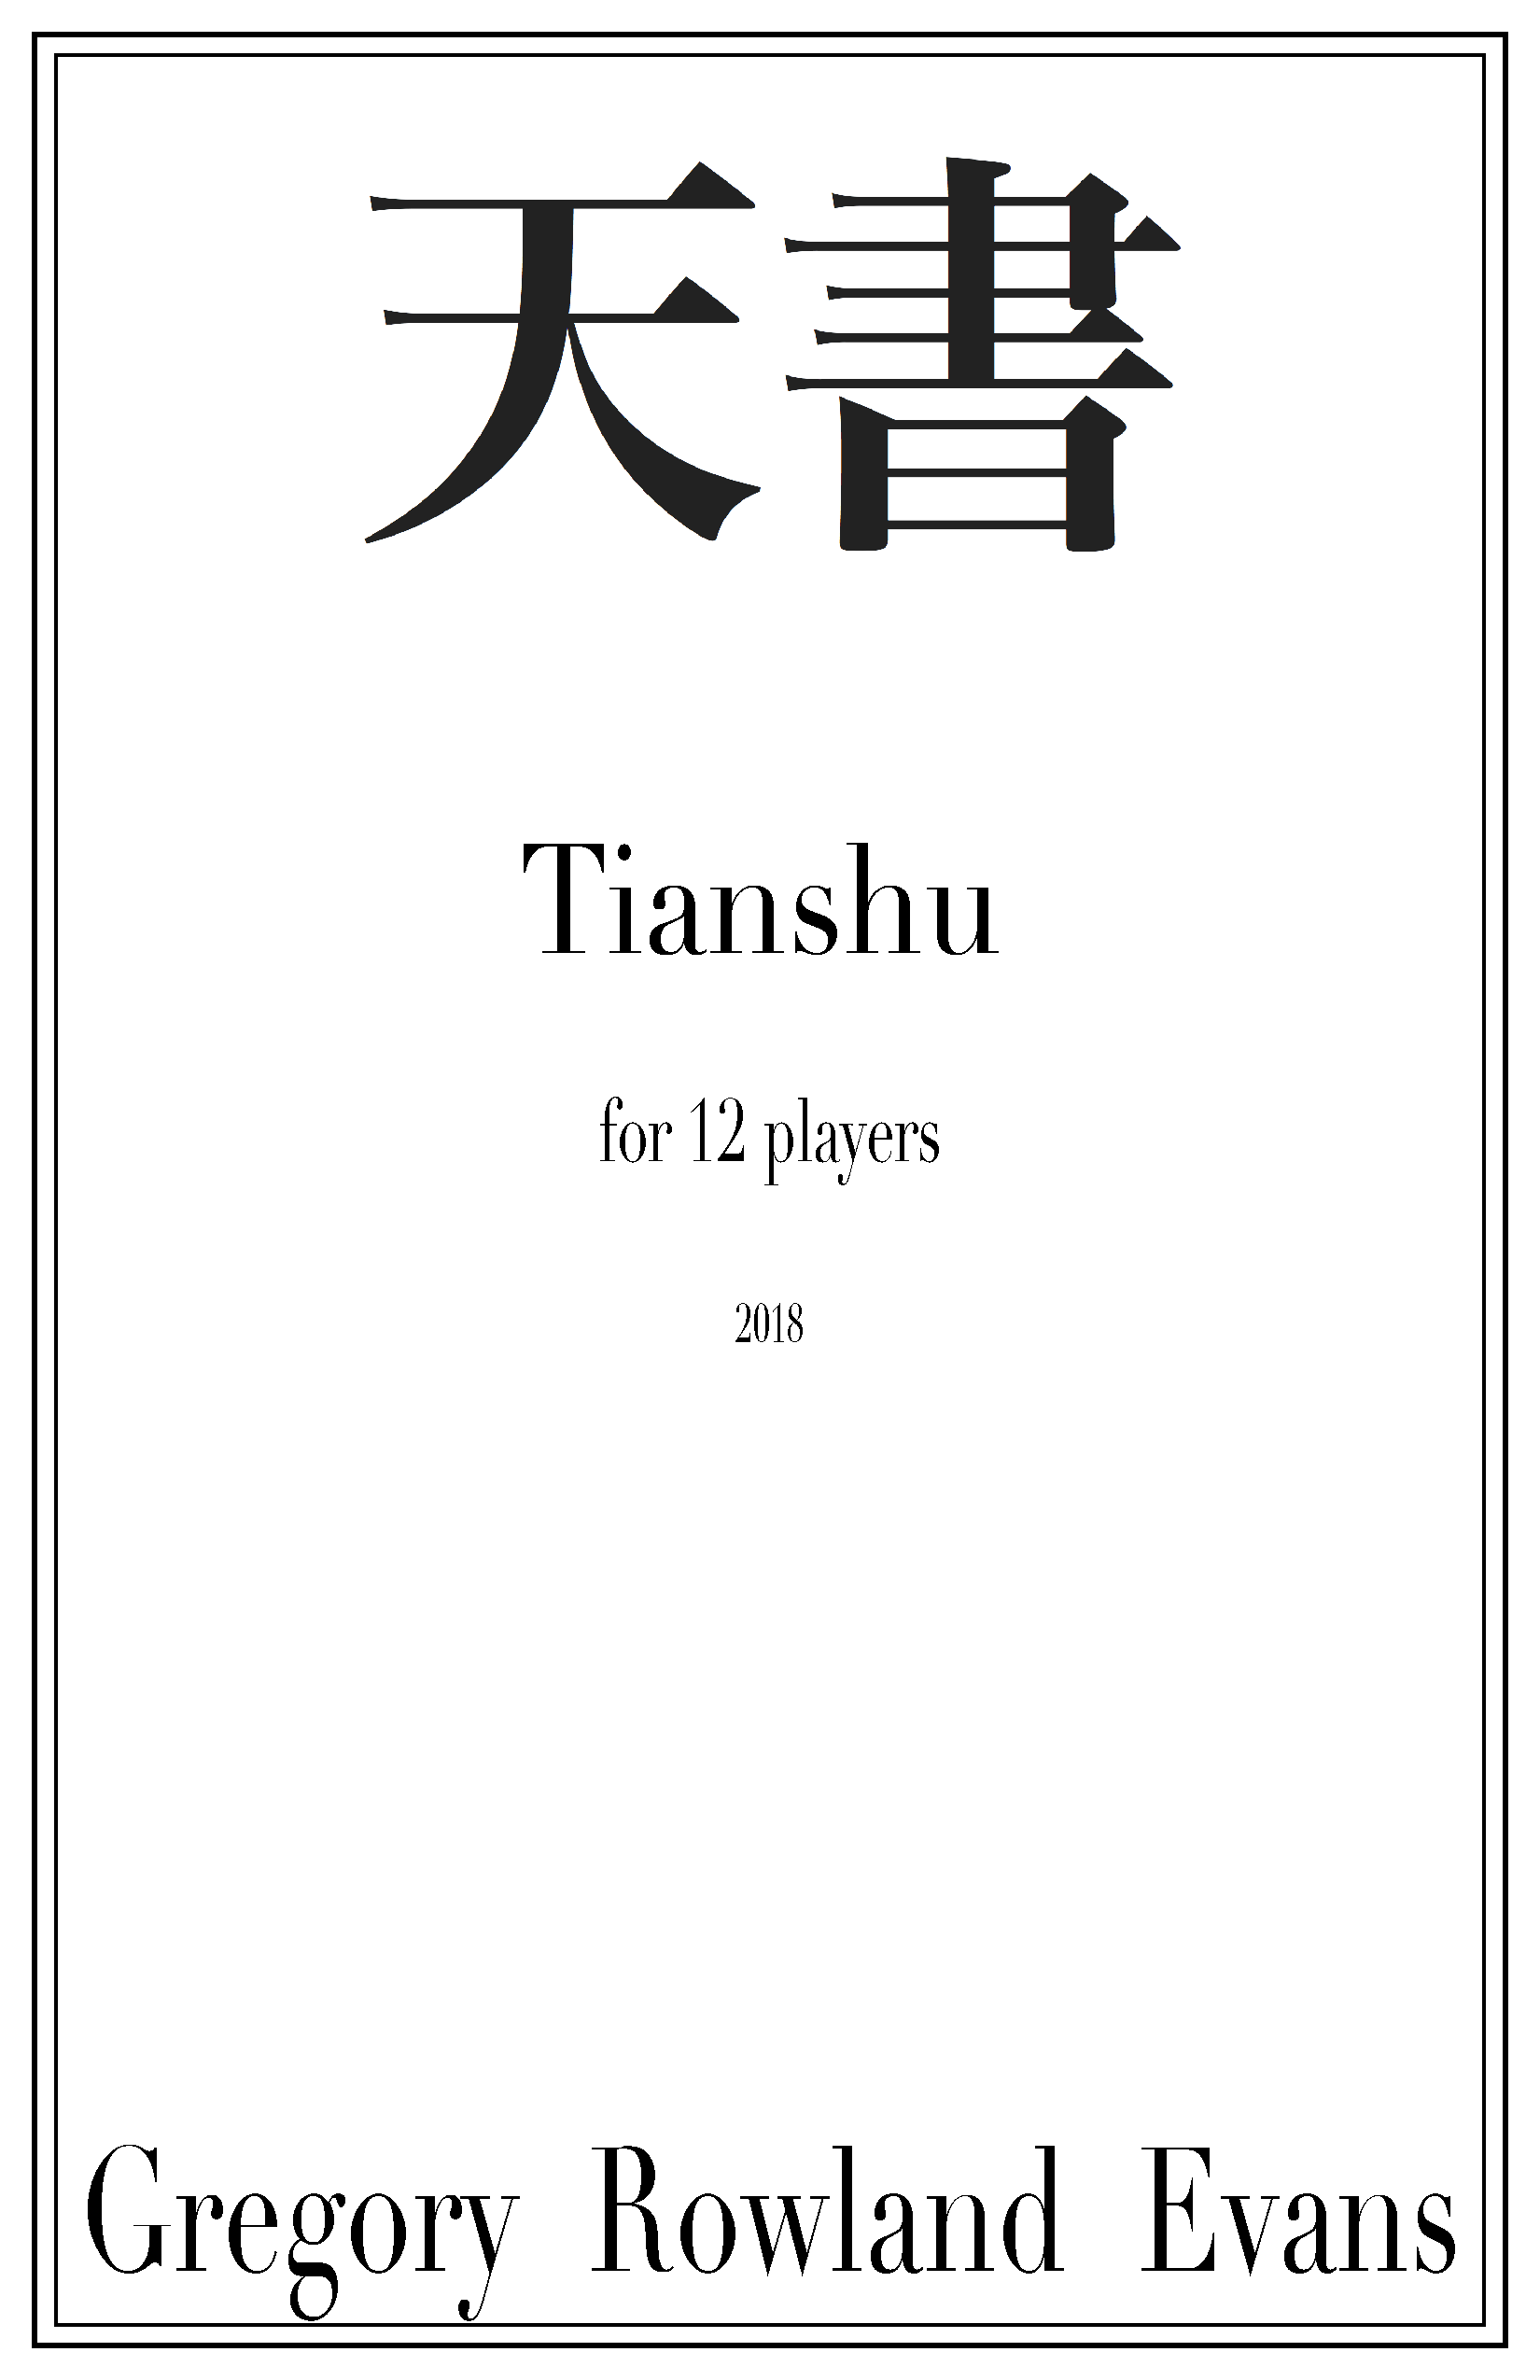
\includepdf[pages=-, pagecommand={},  width=7in,
  height=9.5in, keepaspectratio]{figures/Score/Tianshu_Score.pdf}

\subsection{Four Ages of Sand (for flute, alto saxophone, and violoncello) Score}
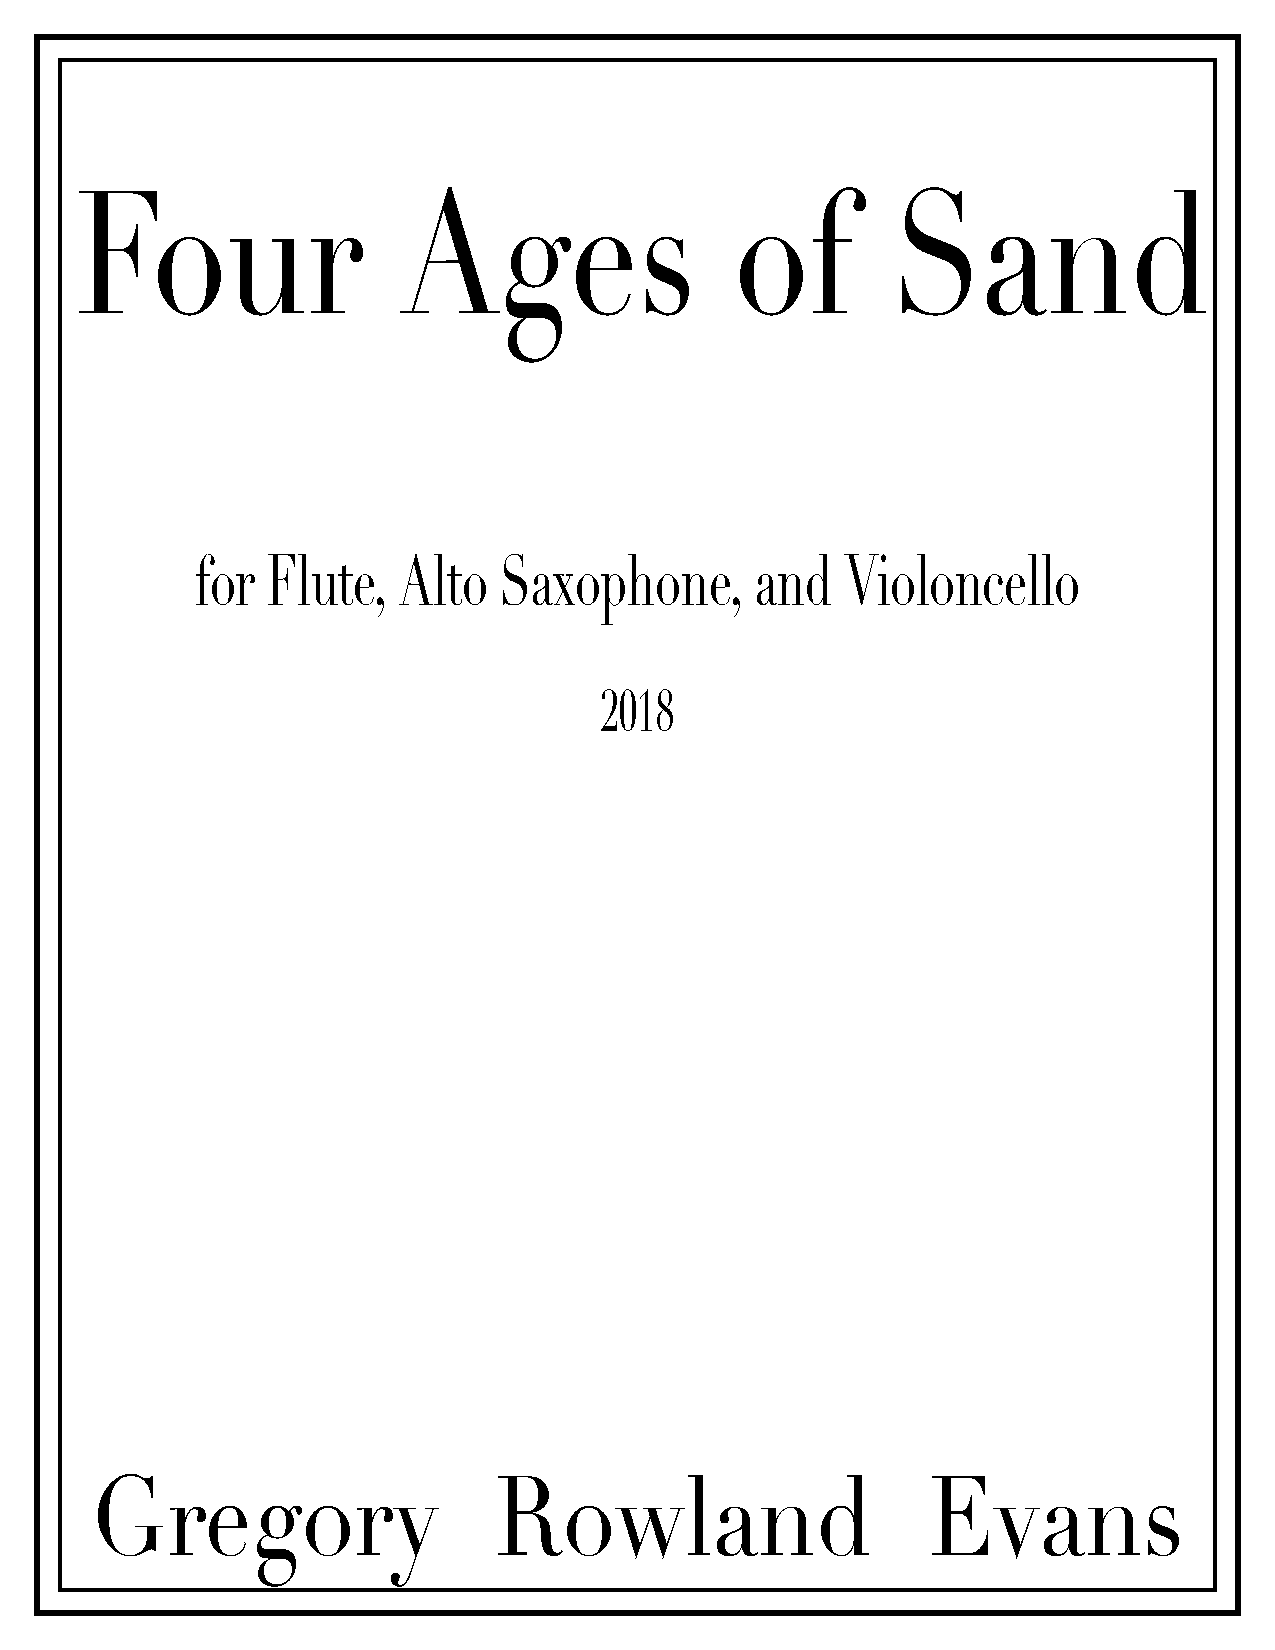
\includepdf[pages=-, pagecommand={},  width=7in,
  height=9.5in, keepaspectratio]{figures/Score/Sand_Score.pdf}